\documentclass[12pt,oneline,a4paper]{ouparticle}

\usepackage{graphicx}
\graphicspath{ {img/} }
\usepackage[labelfont=bf]{caption}
\usepackage{dirtytalk}
\usepackage{hyperref}


\makeatletter
\renewenvironment{table}%
  {\renewcommand{\familydefault}{\ttdefault}\selectfont
  \@float{table}}
  {\end@float}
\makeatother

\newenvironment{localsize}[1]
{%
  \clearpage
  \let\orignewcommand\newcommand
  \let\newcommand\renewcommand
  \makeatletter
  \input{bk#1.clo}%
  \makeatother
  \let\newcommand\orignewcommand
}
{%
  \clearpage
}

\begin{document}

\title{Comparative Analysis of Lock-Based and Lock-Free Concurrent Skiplists with Optimizations for {Get} Operations}

\spacing{1.6}
% \spacing{1.2}

\author{%
\name{Sarang Bhadsavle, Rahul Jaisimha, Nishanth Shanmugham}
\address{The University of Texas at Austin, Austin, TX}
}

\abstract{In this paper we present three implementation of concurrent skiplists: coarse-grained lock-based, fine-grained lock-based, and lock-free. We compare their performance on the three commonly used operations: {\tt get()}, {\tt add()}, and {\tt remove()}. When designing our implementations, we seek to provide an optimization in the fine-grained implementation based on assumptions about the usage of the skiplist; that is, the number of {\tt get()} calls is relatively high and the same key is retrieved more often. Benchmarking the runtime of the implementations shows that our optimized algorithm performs better than coarse-grained versions, and is comparable in performance to non-optimized counterparts as the number of accesses on the skiplist increases.}

\date{November 17, 2016}

% \keywords{skip list; probabilistic data structure}

\maketitle

\section{Introduction}
\label{sec1}

A skiplist, invented in 1990, is a data structure which provides better on-average performance than standard linked lists or balanced trees. As William Pugh claims, skiplists “self-balance” probabilistically rather than strictly, which reduces the overhead that exists in the balancing operation of tree-based data structures \cite{pugh1} \cite{pugh2}. A skiplist's internal structure is shown in Figure \ref{fig:skiplist}. Traversing the bottom level of the skiplist is equivalent to a typical traversal of a linked list. However, the advantage of using a skiplist manifests in the multi-layer aspect of the structure. By starting from the top left of the list and traveling right and down appropriately, nodes can effectively be {\it skipped}, which results in better performance when searching for a node.

\begin{figure}
    \centering
    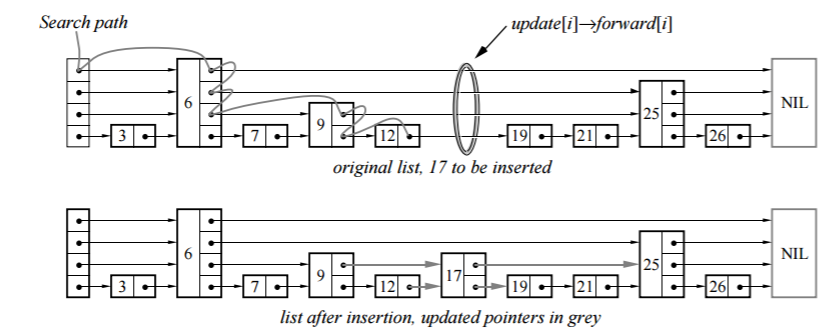
\includegraphics[width=\textwidth]{skiplist}
    \caption{Skiplist add operation \cite{pugh1}}
    \label{fig:skiplist}
\end{figure}

\section{Algorithms}

We developed three concurrent skiplist implementations in Java: coarse-grained, fine-grained lock-based, and lock-free. 
The inherent nature of skiplists lends itself well to designing concurrent versions of the data structure. The coarse-grained implementation uses locks around the {\tt get()}, {\tt add()}, and {\tt remove()} functions to guarantee mutual exclusion. However, more concurrent access to the list is often desirable, which is motivation for the fine-grained lock-based and lock-free versions of the data structure. When designing algorithms for these versions, we make use of the concepts of optimism and laziness as described by Heller et al. [4] and as implemented in the {\tt ConcurrentSkipListMap} class in the Java standard library. For instance, when mutating operations such as {\tt add()} and {\tt remove()} are happening concurrently, a node is initially marked as deleted and only later physically deleted. 

 The fine-grained lock-based algorithm we chose to implement is presented by M. Herlihy et. al \cite{provably} which utilizes the concepts of optimism and laziness. We also implemented Herlihy and Shavit’s lock-free implementation \cite{art} which uses similar principles to the fine-grained lock-based algorithm in terms of laziness. In addition to the above implementation, we also attempted to optimize the fine-grained algorithm for a specific circumstance described in the next section.

In all of our implementations, nodes have a probability of 0.5 to increase in height when added to the skiplist. This makes every level contain half as many expected entries as the level below it. This works out to giving the skiplist a height of $log_{2}N$ where $N$ is the capacity of the data structure. Predetermining this value helps in implementing performant skiplists: we chose $N={\tt2^{32}}$ and maximum height = {\tt 32}. 

\section{Optimizations}
Besides the standard versions above, we implement a modified version fine-grained skiplist to optimize performance in the case of repeated {\tt get()} of the same entry. We make the following hypothesis:


\say{If a particular entry {\it k} in the skiplist is searched for in at least half of the {\tt get()} operations and if the majority of calls to the skiplist are {\tt get()} operations, then improving the performance of the {\tt get()} operation for {\it k} will improve the overall performance.}

\subsection{Approach}

For each invocation of {\tt get()}, we give the retrieved entry a 10\% chance of increasing in height. The aim is that the increasing the height makes the entry quicker to retrieve in future calls to {\tt get()}. We chose a 10\% chance for the following reason: In a typical usage scenario for a map ({90\% get, 9\% add, 1\% remove}), the 10\% probability is expected to increase the height of an entry every 10 calls to {\tt get()}. An entry that entry is retrieved retrieved more often is expected to be the highest, thus making future get() operations for it faster. 

It also worth noting that using the 10\% probability also helps handle the case in which an entry's level may grow too high since the height is expected to increase only 1 out of 10 times.

\section{Performance}

We benchmarked the running time of the above algorithms implementing them in the Java programming language. We also include the standard libary's {\tt ConcurrentSkipListMap} for comparison. We implemented all the described algorithms use a {\tt String} key and a {\Integer} value for the skiplist entries. There are at most 100 keys and 32 levels. To understand time complexities, we ran our tests for differing numbers of get, put, and remove operations. We vary the number of operations performed (10, 100, 1000) and the number of threads (1, 10, 100). To ensure that the JVM is warmed up, we averaged each final result over 5 runs.

We also vary the relative percentage of {\tt get()}, {\tt add()}, and {\tt remove()} in the following ratios to observe how the implementations vary under different access patterns:

\begin{itemize}
\itemsep0em 
    \item { 90\% get, 9\% add, 1\% remove}
    \item { 70\% get, 20\% add, 10\% remove}
    \item { 0\% get, 50\% add, 50\% remove}
\end{itemize}

\subsection{Environment}

The benchmarking environment has the following specifications:

\begin{itemize}
\itemsep0em 
    \item JDK 1.8.0\_101
    \item 2.4GHz Intel Core i5 processor
    \item 8GB of 1600MHz DDR3 RAM
    \item Macbook Pro Retina, Late 2013
\end{itemize}


\subsection{Results}

The Figures 2--5 present the results grouped by their relative uses of the {\tt get}, {\tt add}, and {\tt remove} functions. For 10 operations, the tests are mainly circumstantial and the outputs are are inconclusive even when the tests are averaged over many runs. For 100 or 1000 operations it is easy to see how the algorithms fare, with the Java standard library implementation consistently outperforming the other implementations for any number of threads. Another key takeaway is the consistent pattern of the non-optimized fine-grained lock-based skiplist (denoted as “fine0”) doing at least as well as the coarse-grained lock-based skiplist (denoted as “coarse0”).

For randomly chosen keys in the range 0..99, the optimized version of our fine-grained skiplist (denoted as “fine1”) performed almost as well as the non-optimized version (denoted as “fine0”). These results are presented in Figures 2,3,4.

In the other case in which the same key is retrieved 50\% of the time, the optimized version performs better than the non-optimized version for 1000 operations and 100 threads, but not as significantly as we expected (Figure \ref{fig:g4}). This is likely due to the overhead of placing a lock on retrieved objects while increasing its height to ensure thread-safety. Further benchmarking is required to verify this.

Appendix A lists the raw data from the benchmarks.

\begin{figure}
    \centering
    \hspace*{-2.25cm}
    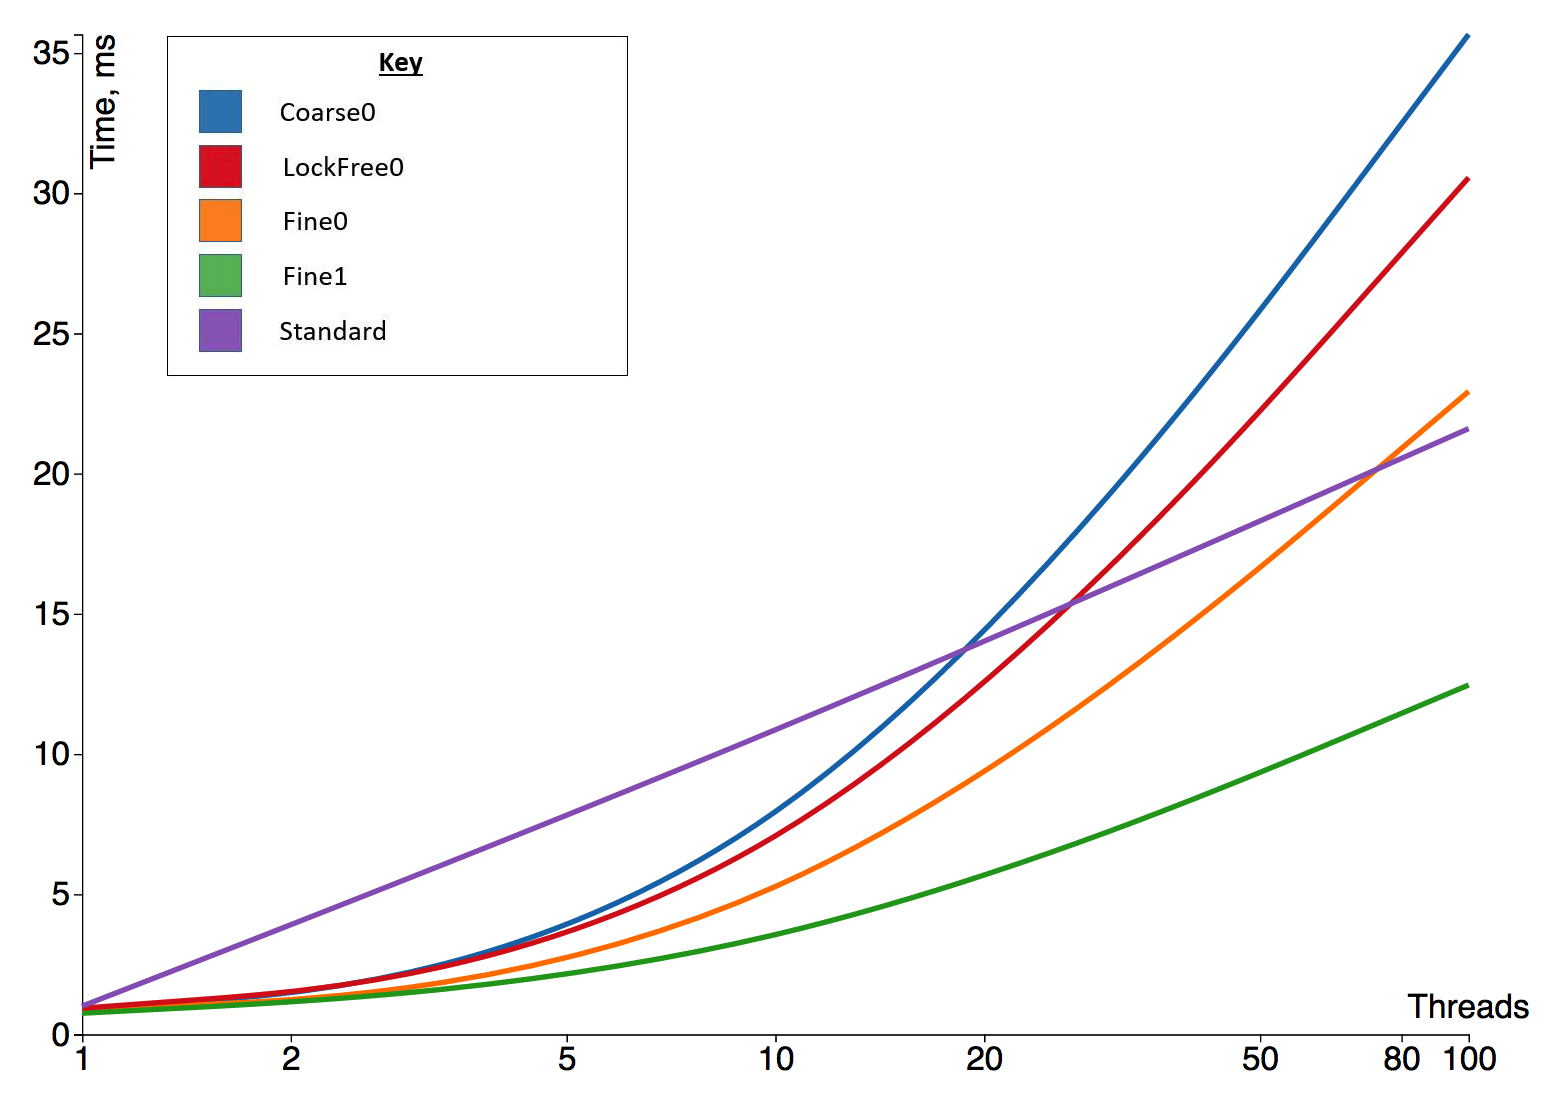
\includegraphics[width=0.37\linewidth]{1}\hspace{0em}
    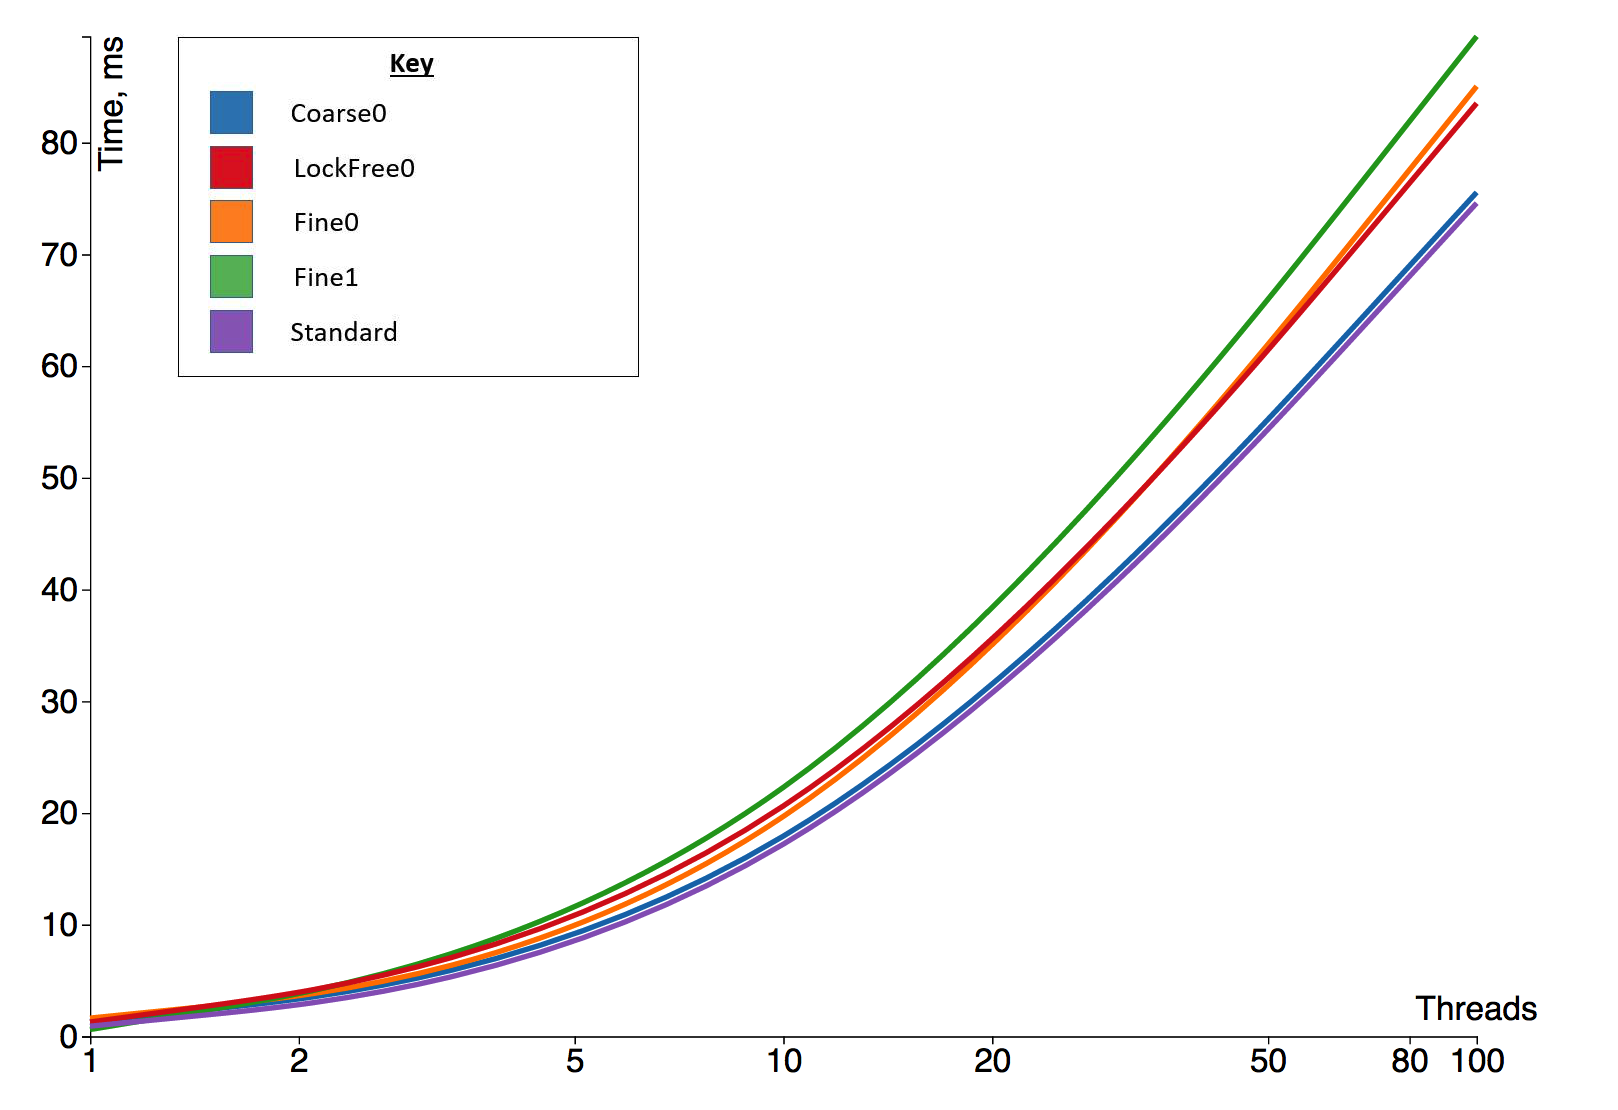
\includegraphics[width=0.37\linewidth]{2}\hspace{0em}
    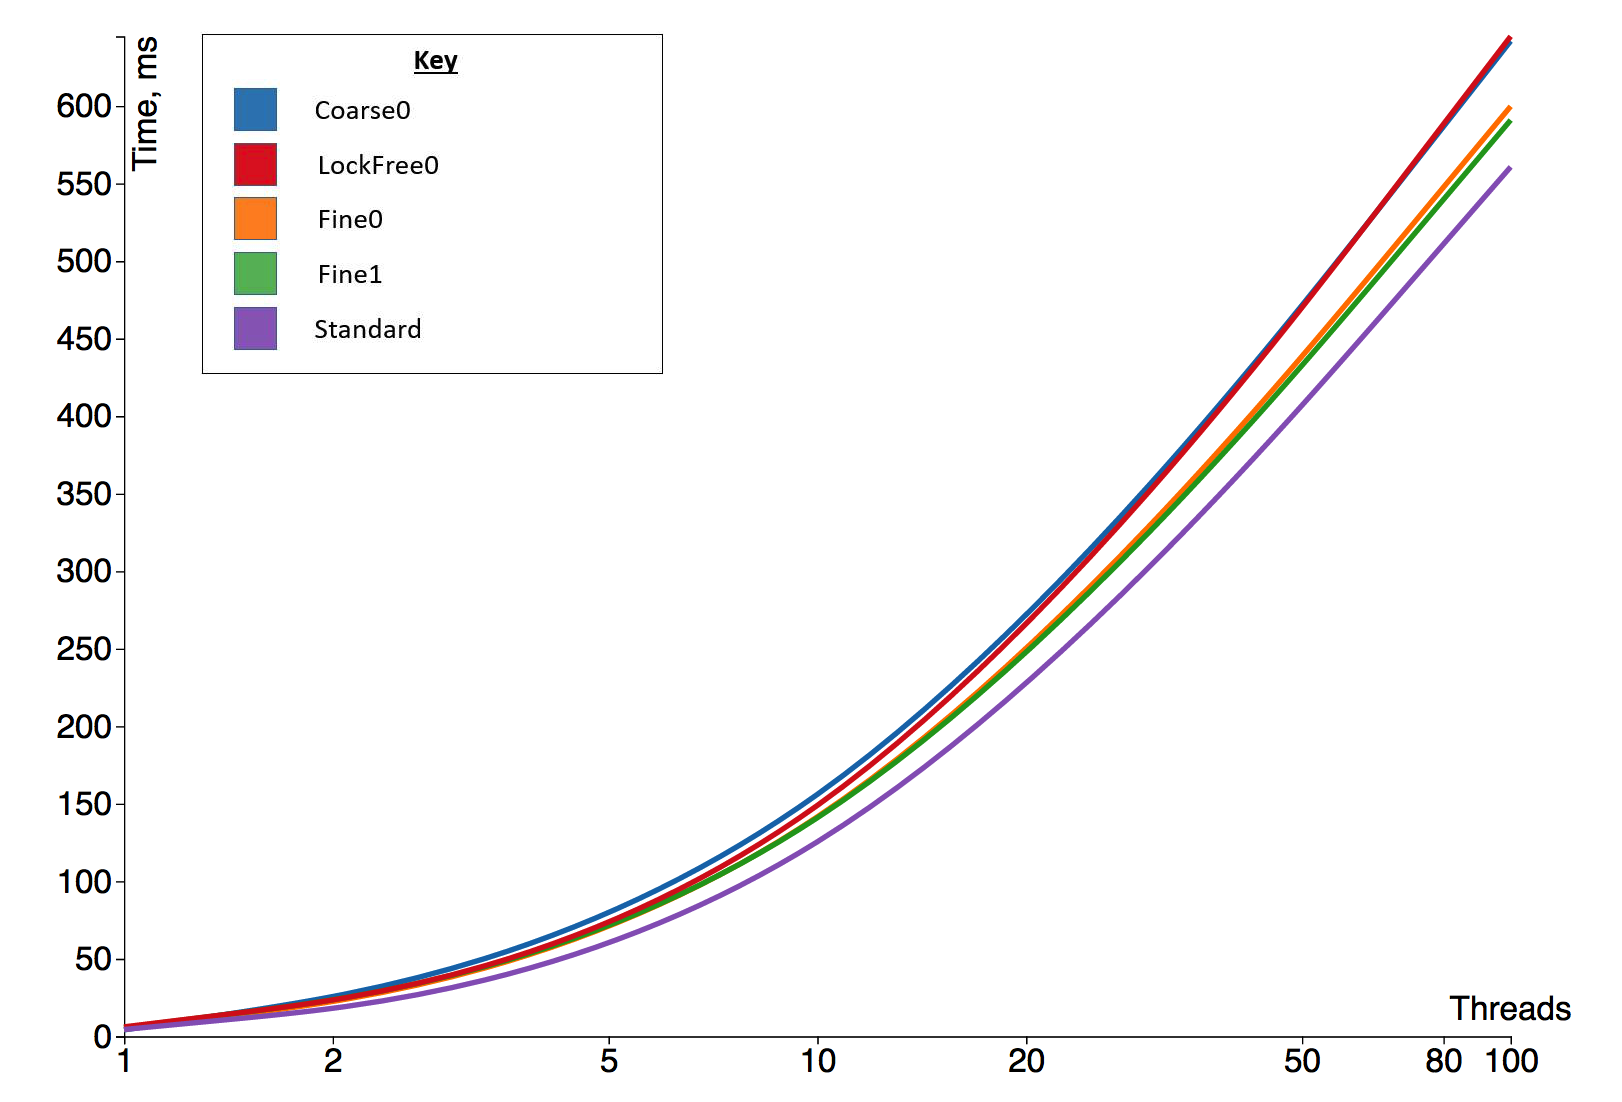
\includegraphics[width=0.37\linewidth]{3}
    \hspace*{-2.25cm}
    \centering
    \caption{Time v. number of threads (0\% get, 50\% add, 50\% remove operations).\newline{}
    {\it From left to right: 10 operations, 100 operations, 1000 operations.}}
    \label{fig:g1}
\end{figure}

\begin{figure}
    \centering
    \hspace*{-2.25cm}
    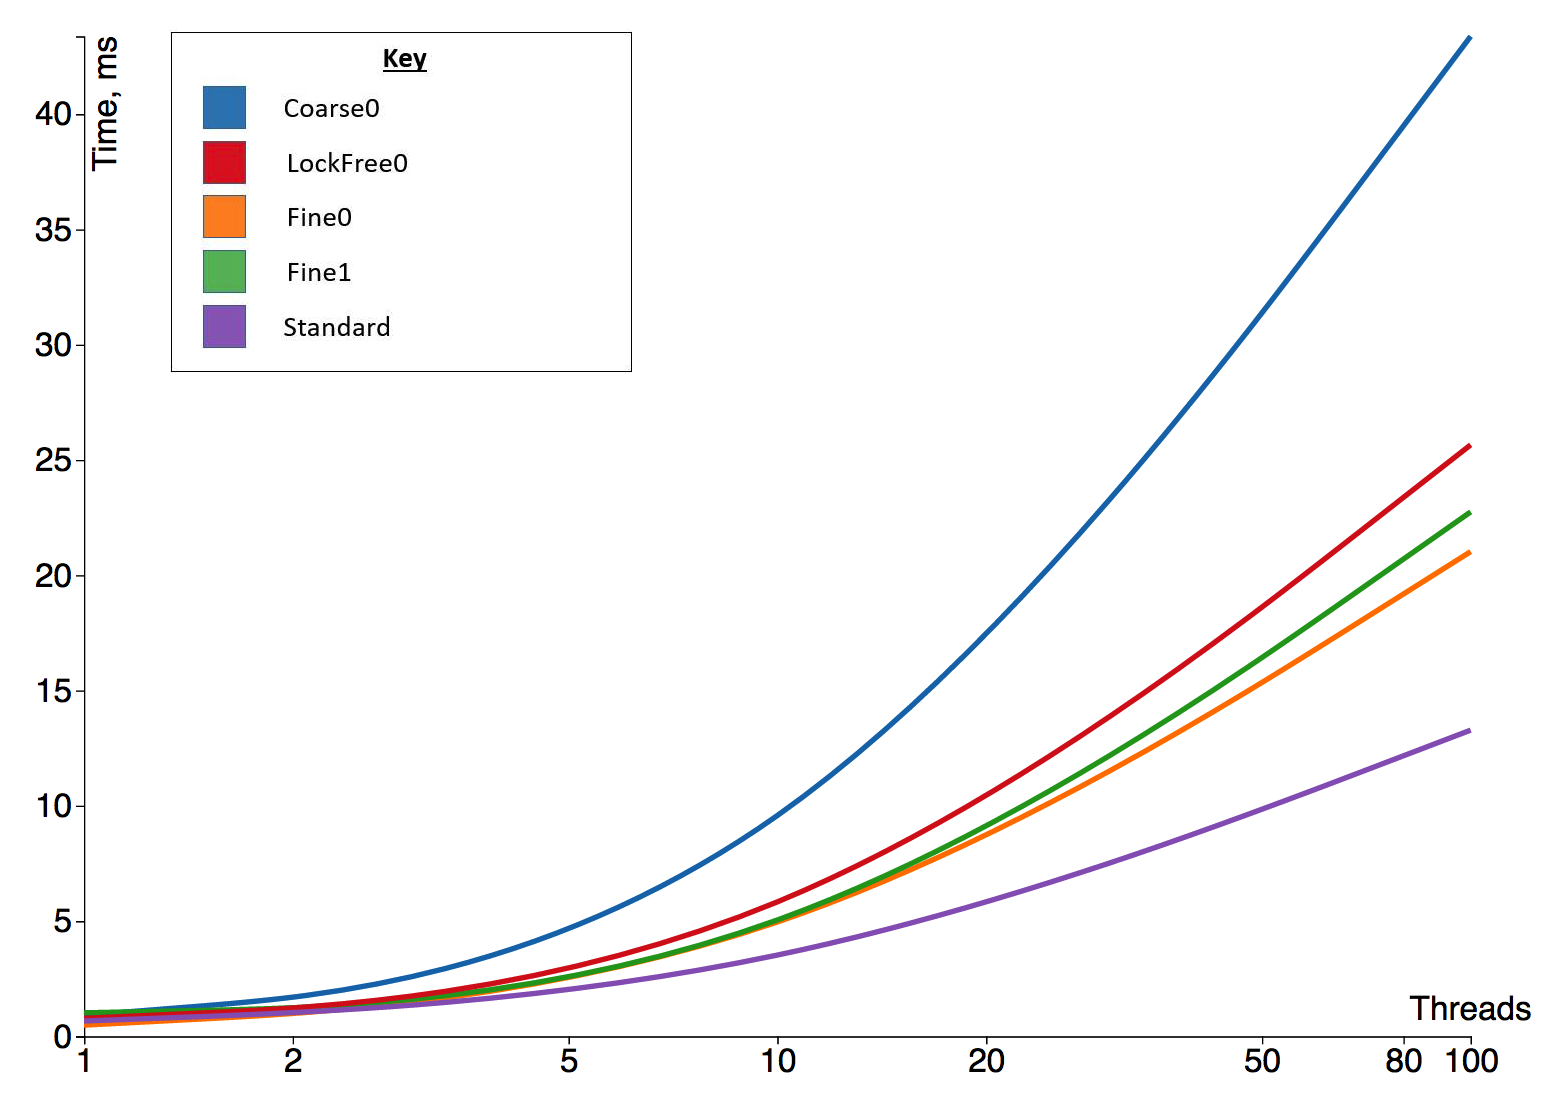
\includegraphics[width=0.37\linewidth]{4}\hspace{0em}
    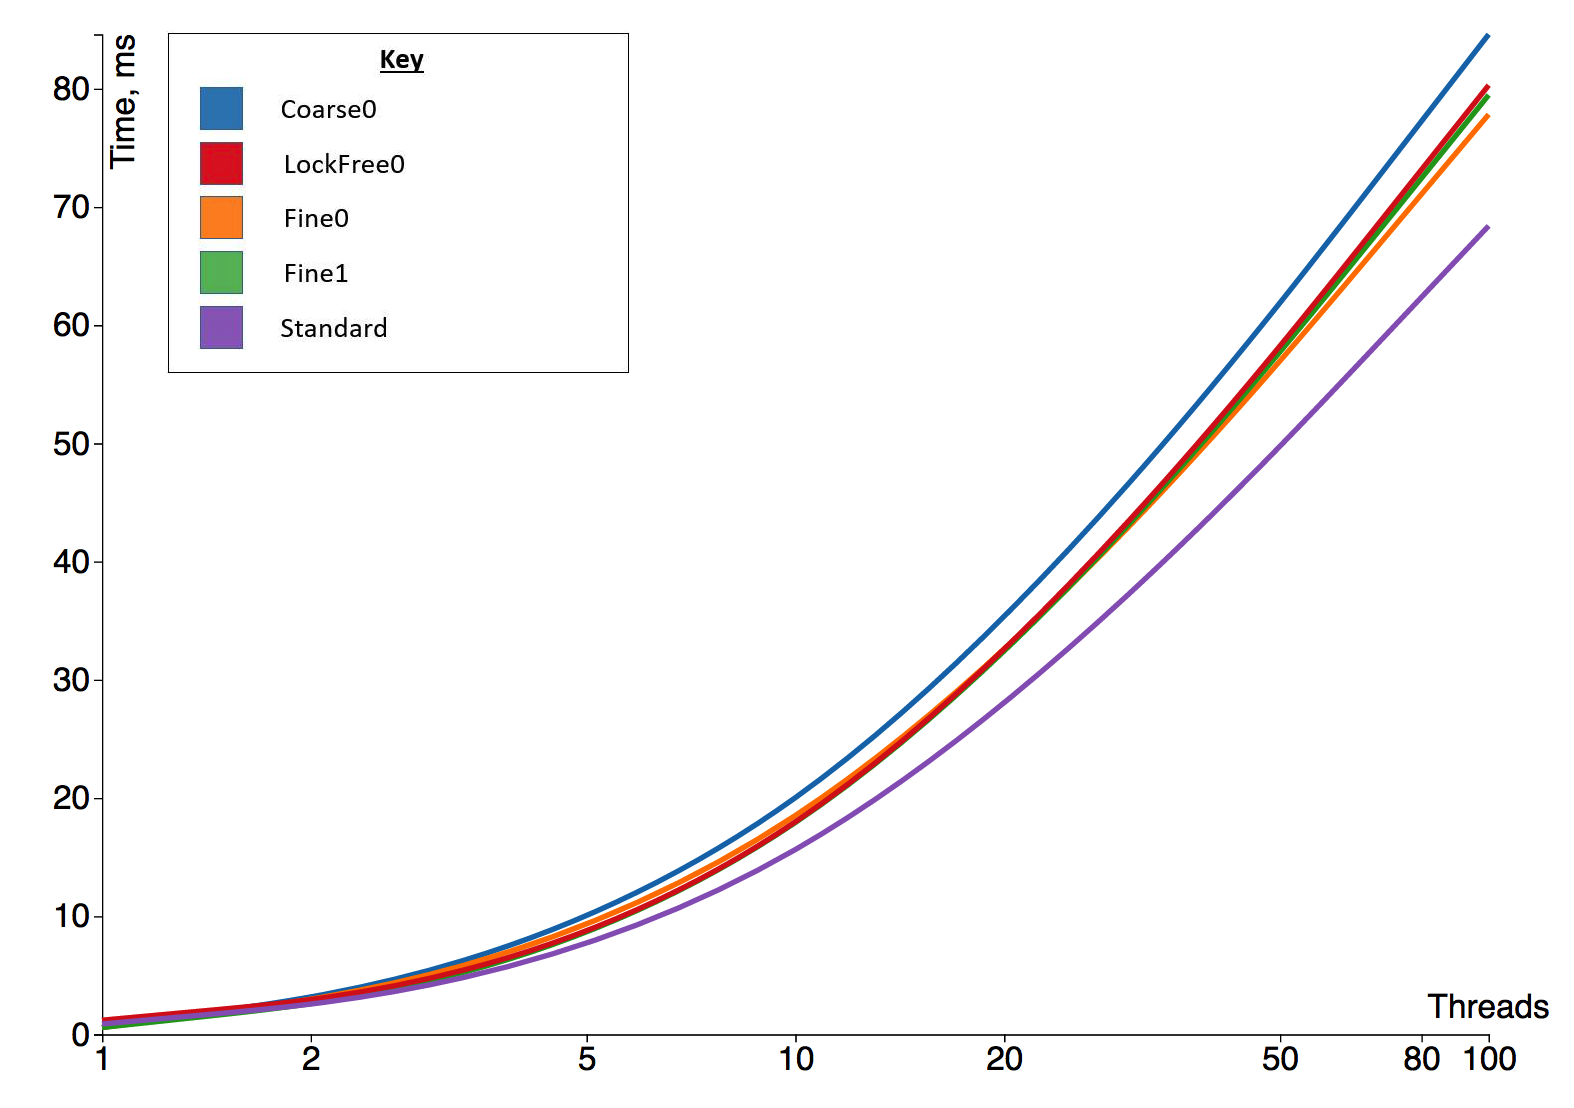
\includegraphics[width=0.37\linewidth]{5}\hspace{0em}
    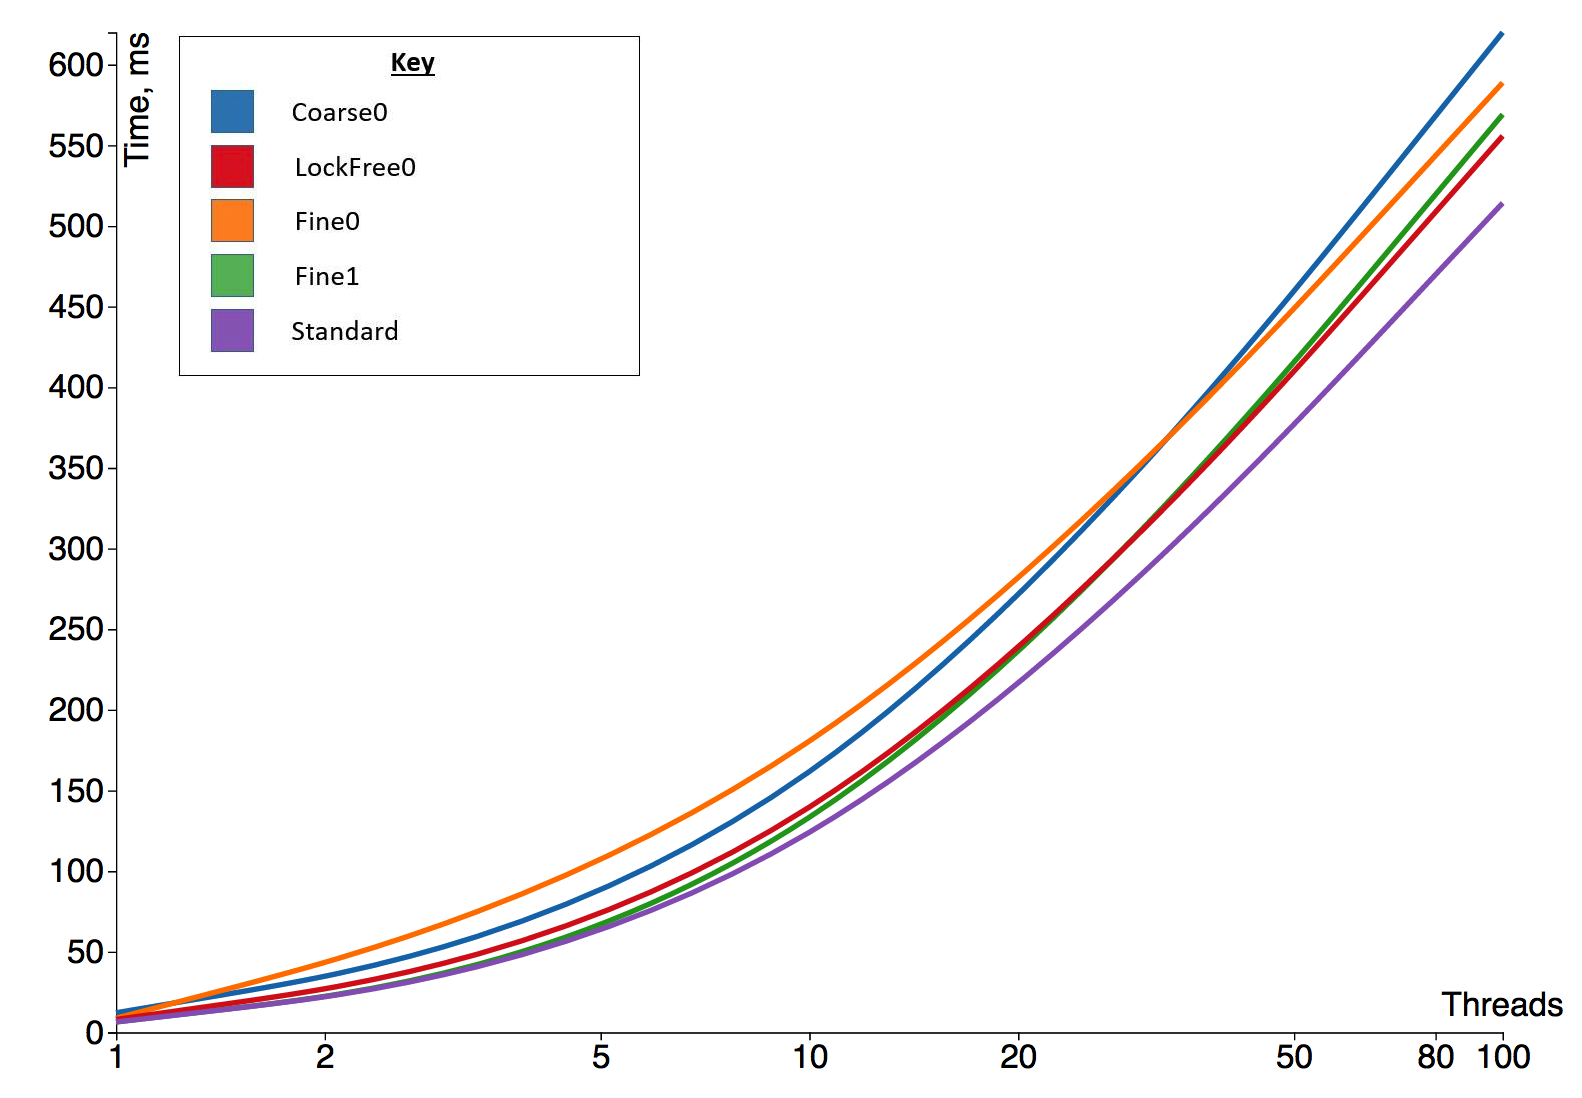
\includegraphics[width=0.37\linewidth]{6}
    \hspace*{-2.25cm}
    \centering
    \caption{Time v. number of threads (70\% get, 20\% add, 10\% remove operations).\newline{}
    {\it From left to right: 10 operations, 100 operations, 1000 operations.}}
    \label{fig:g2}
\end{figure}

\begin{figure}
    \centering
    \hspace*{-2.25cm}
    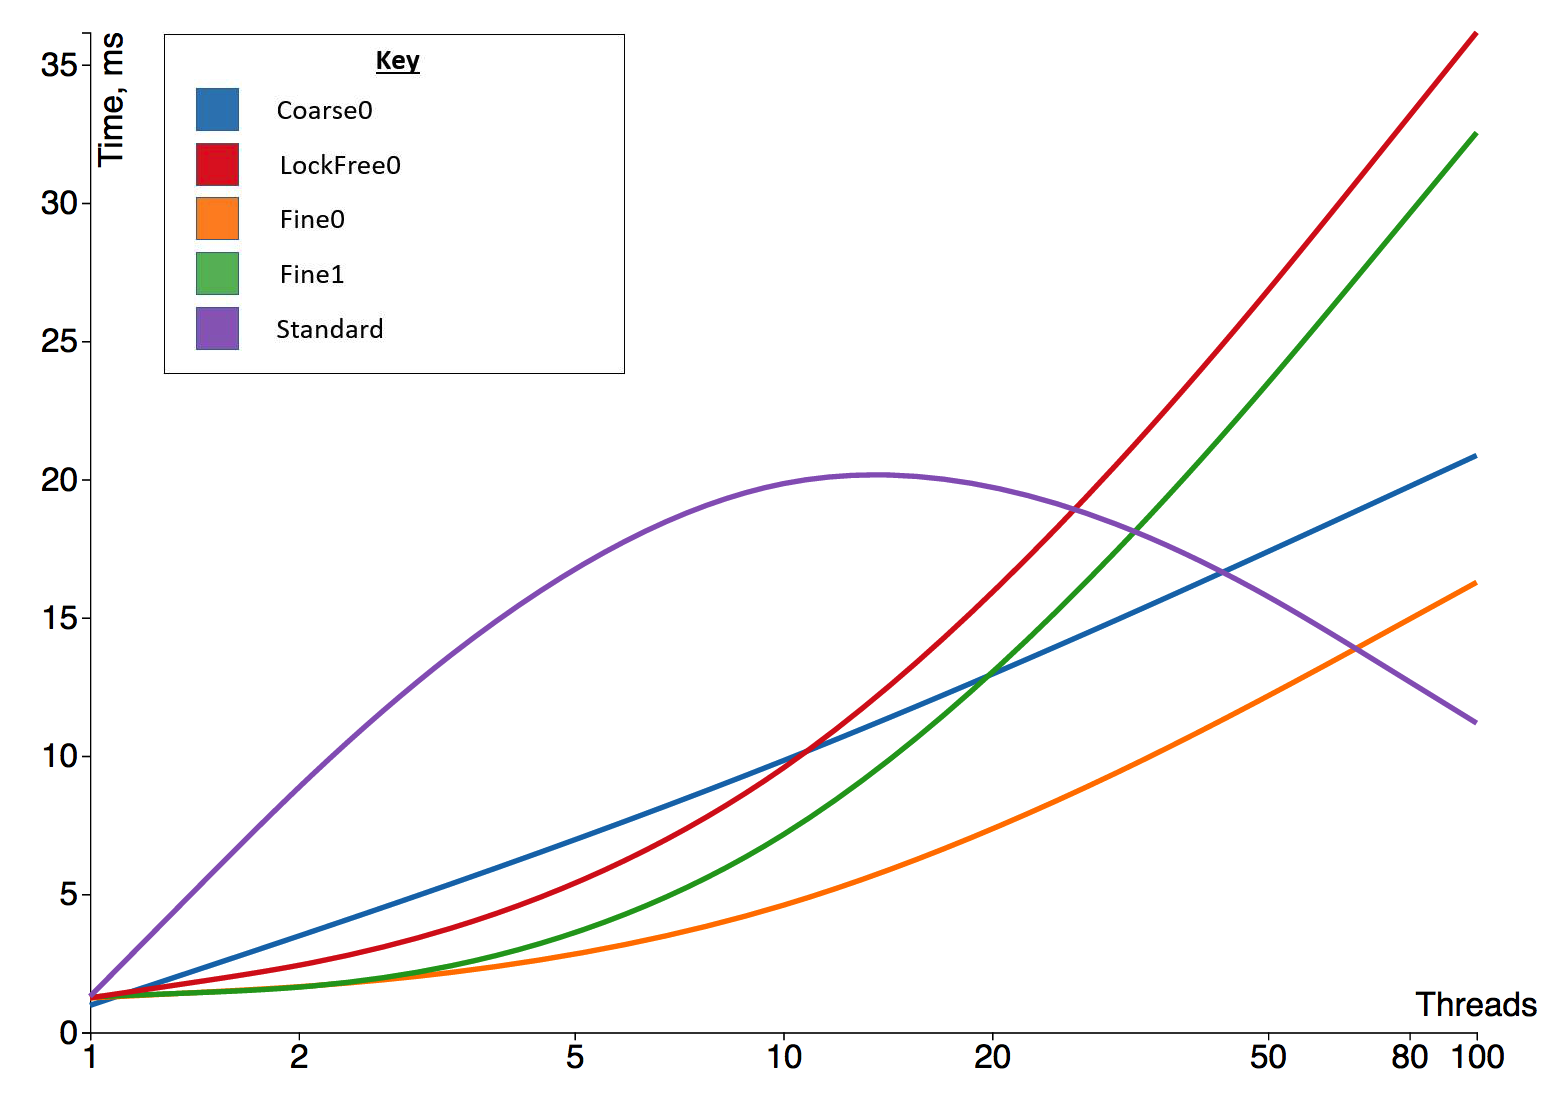
\includegraphics[width=0.37\linewidth]{7}\hspace{0em}
    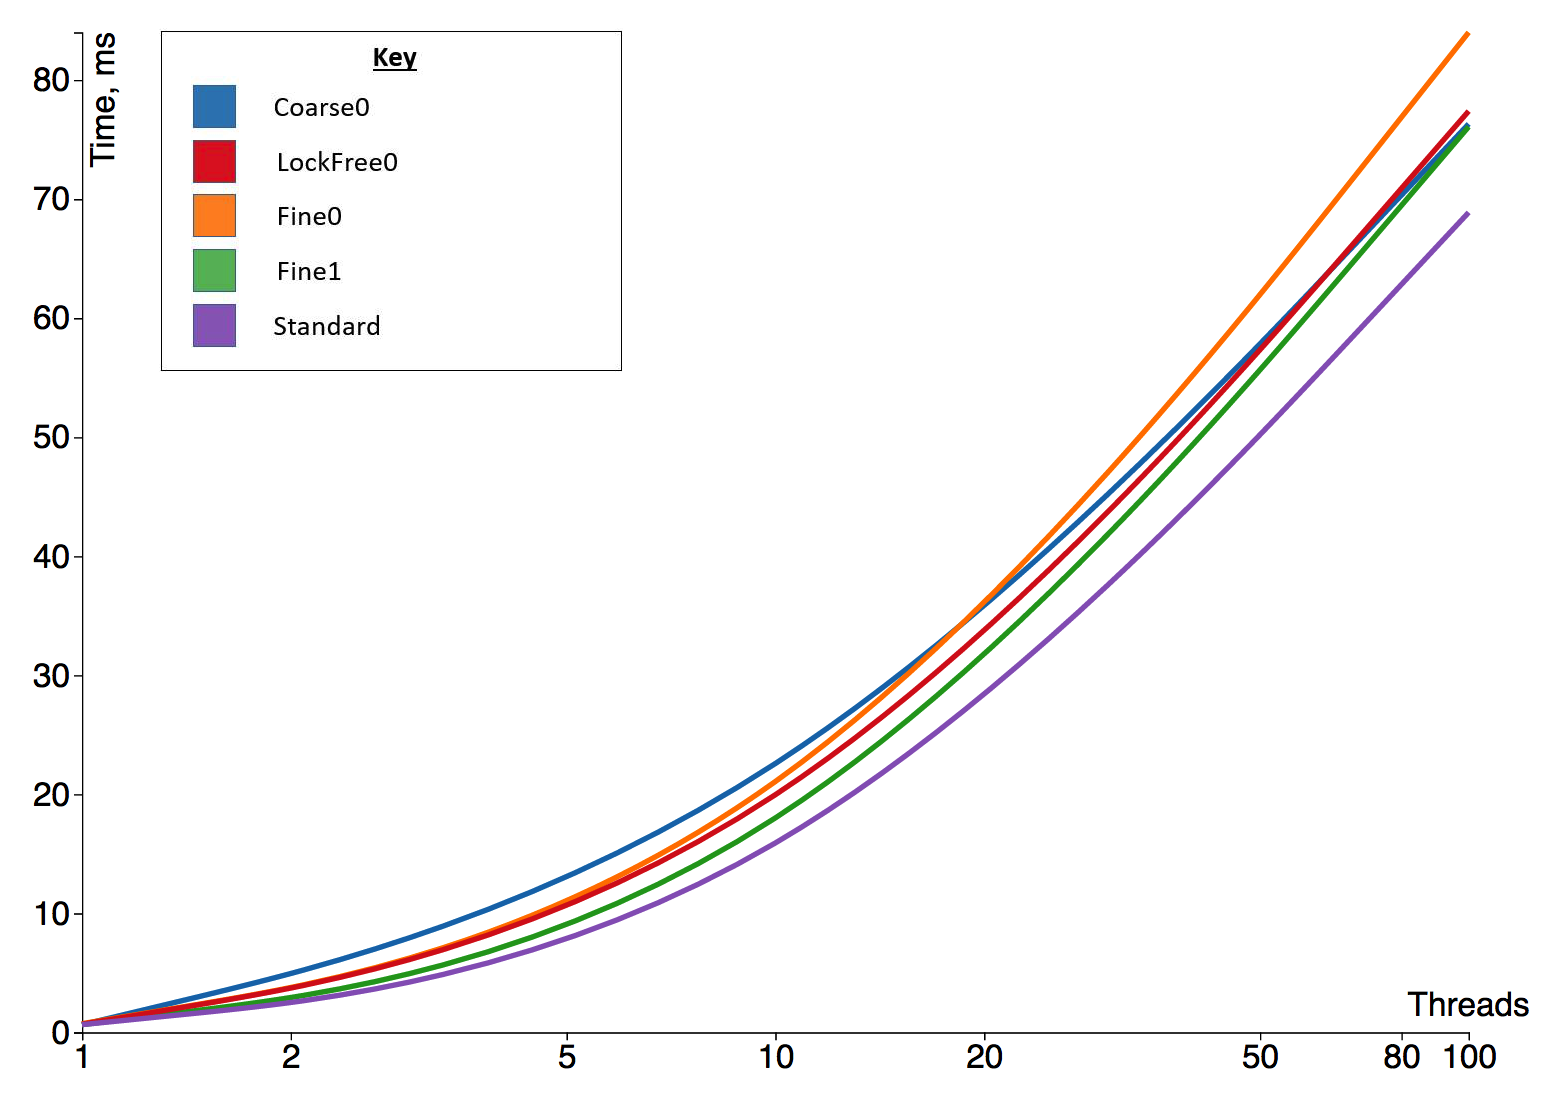
\includegraphics[width=0.37\linewidth]{8}\hspace{0em}
    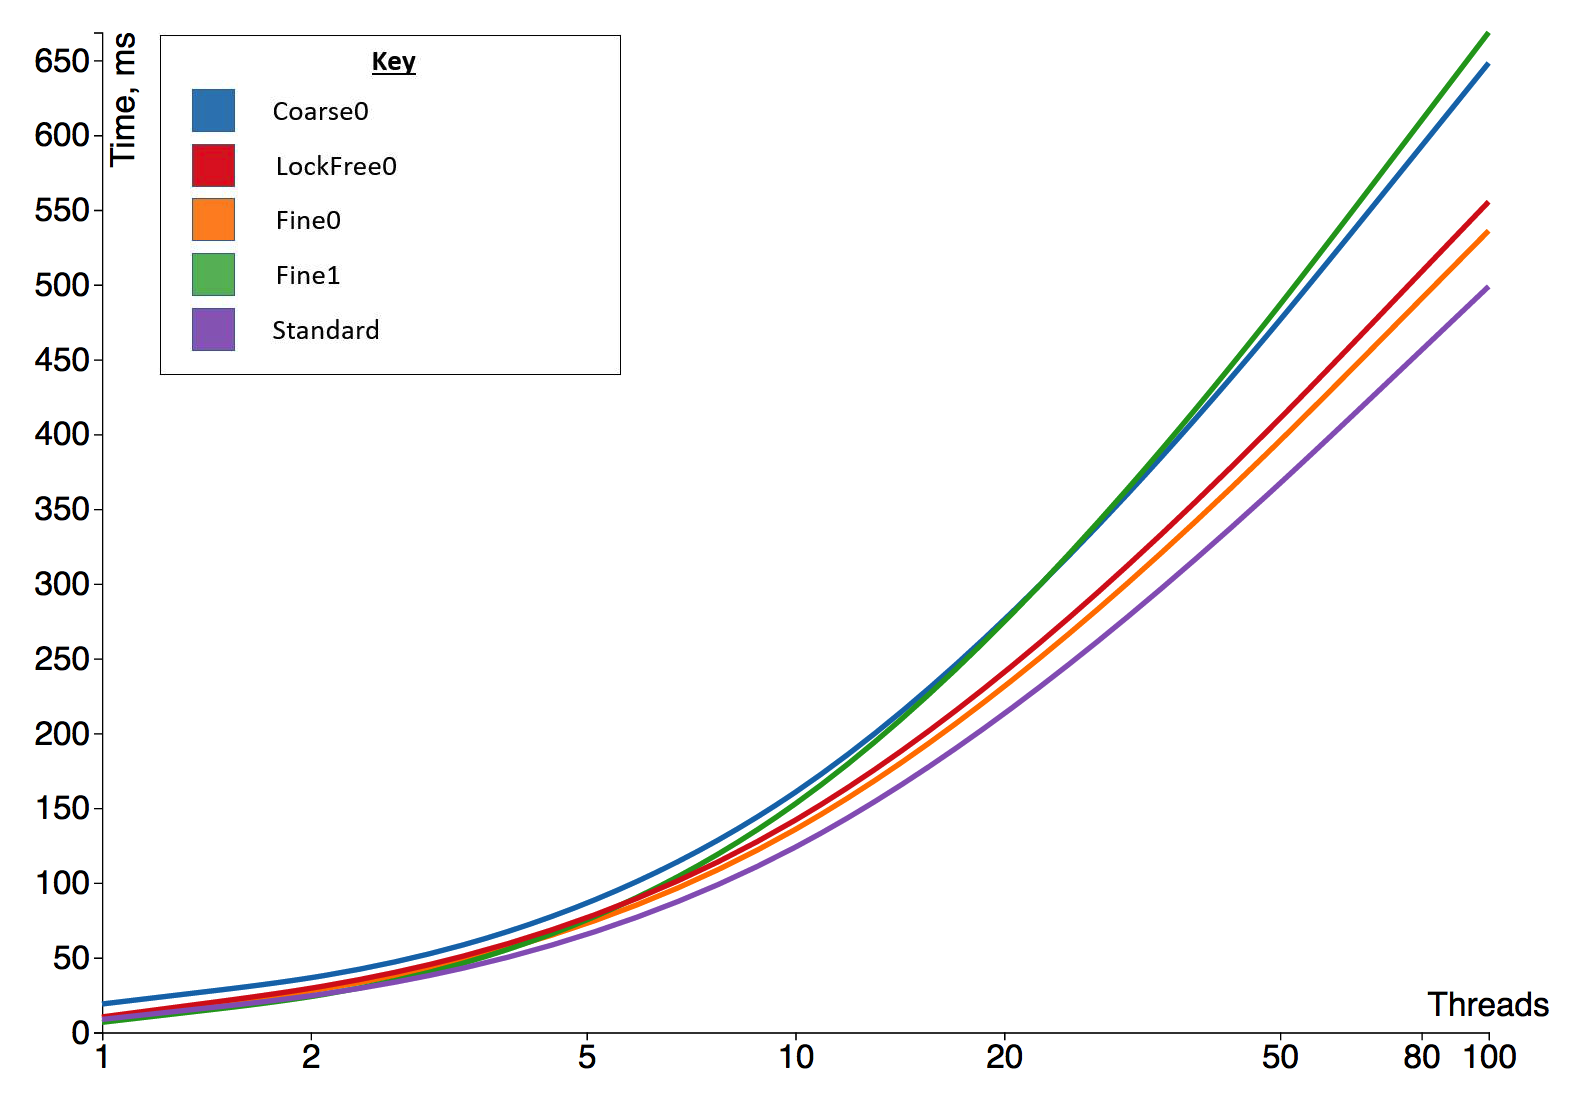
\includegraphics[width=0.37\linewidth]{9}
    \hspace*{-2.25cm}
    \centering
    \caption{Time v. number of threads (90\% get, 9\% add, and 1\% remove operations).\newline{}
    {\it From left to right: 10 operations, 100 operations, 1000 operations.}}
    \label{fig:g3}
\end{figure}

\begin{figure}
   \centering
    \hspace*{-2.25cm}
    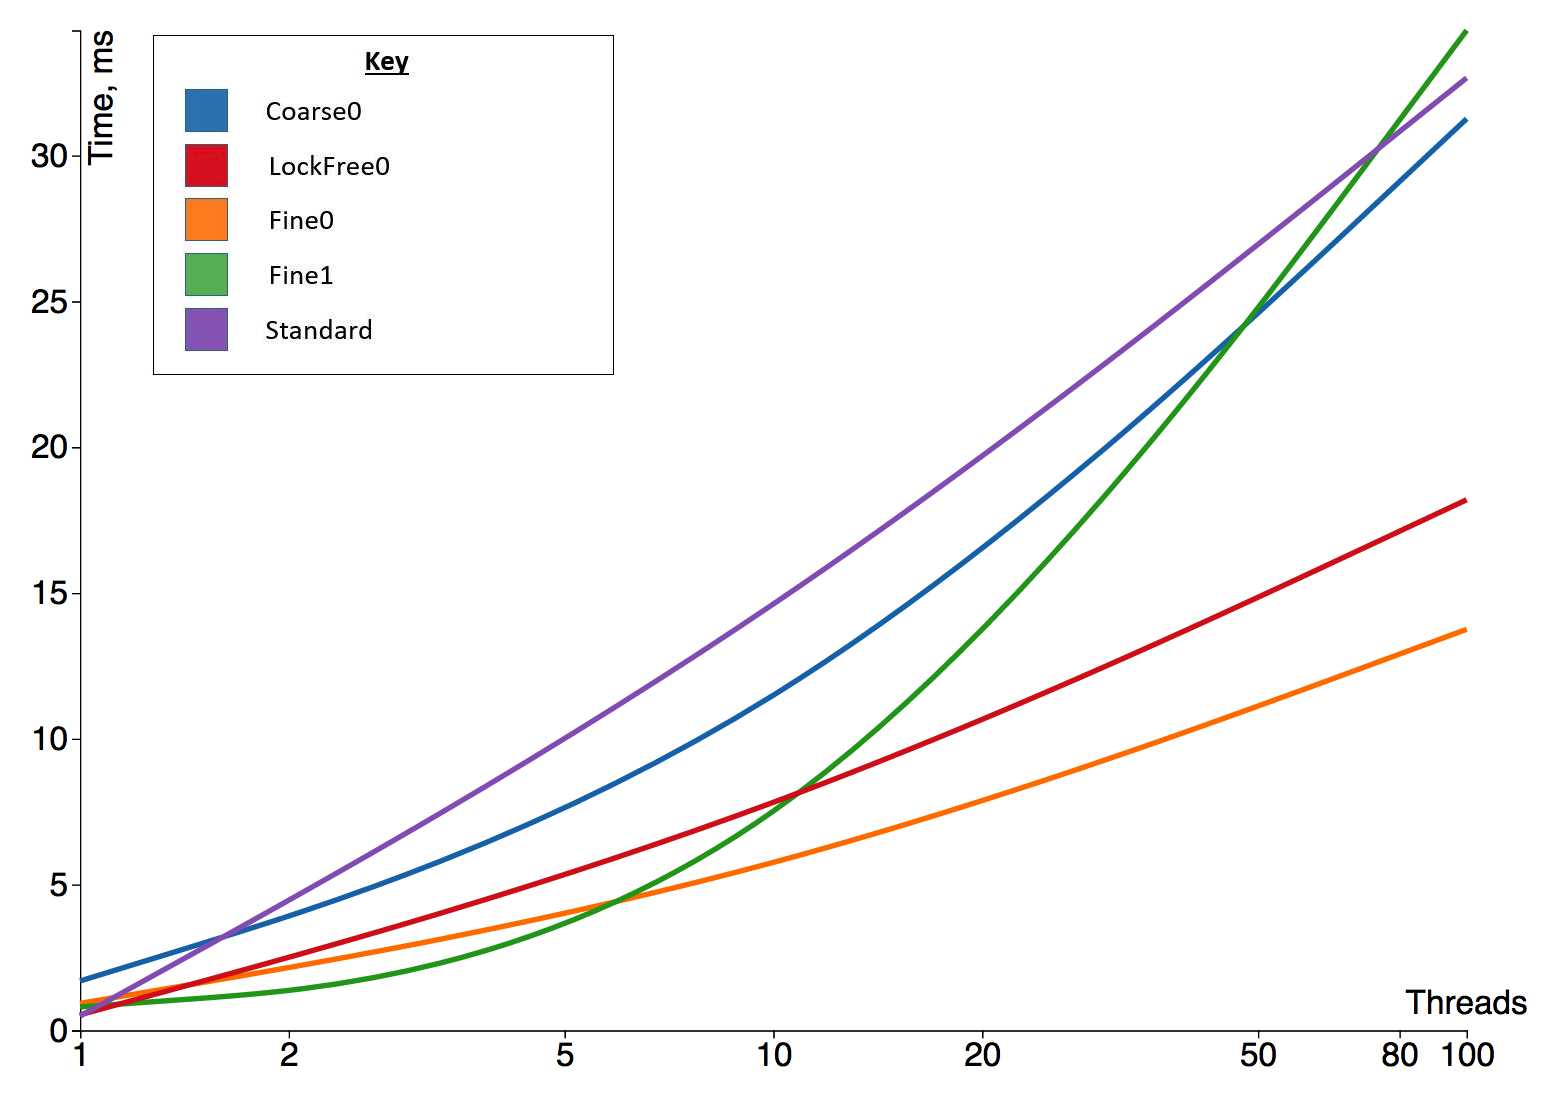
\includegraphics[width=0.37\linewidth]{10}\hspace{0em}
    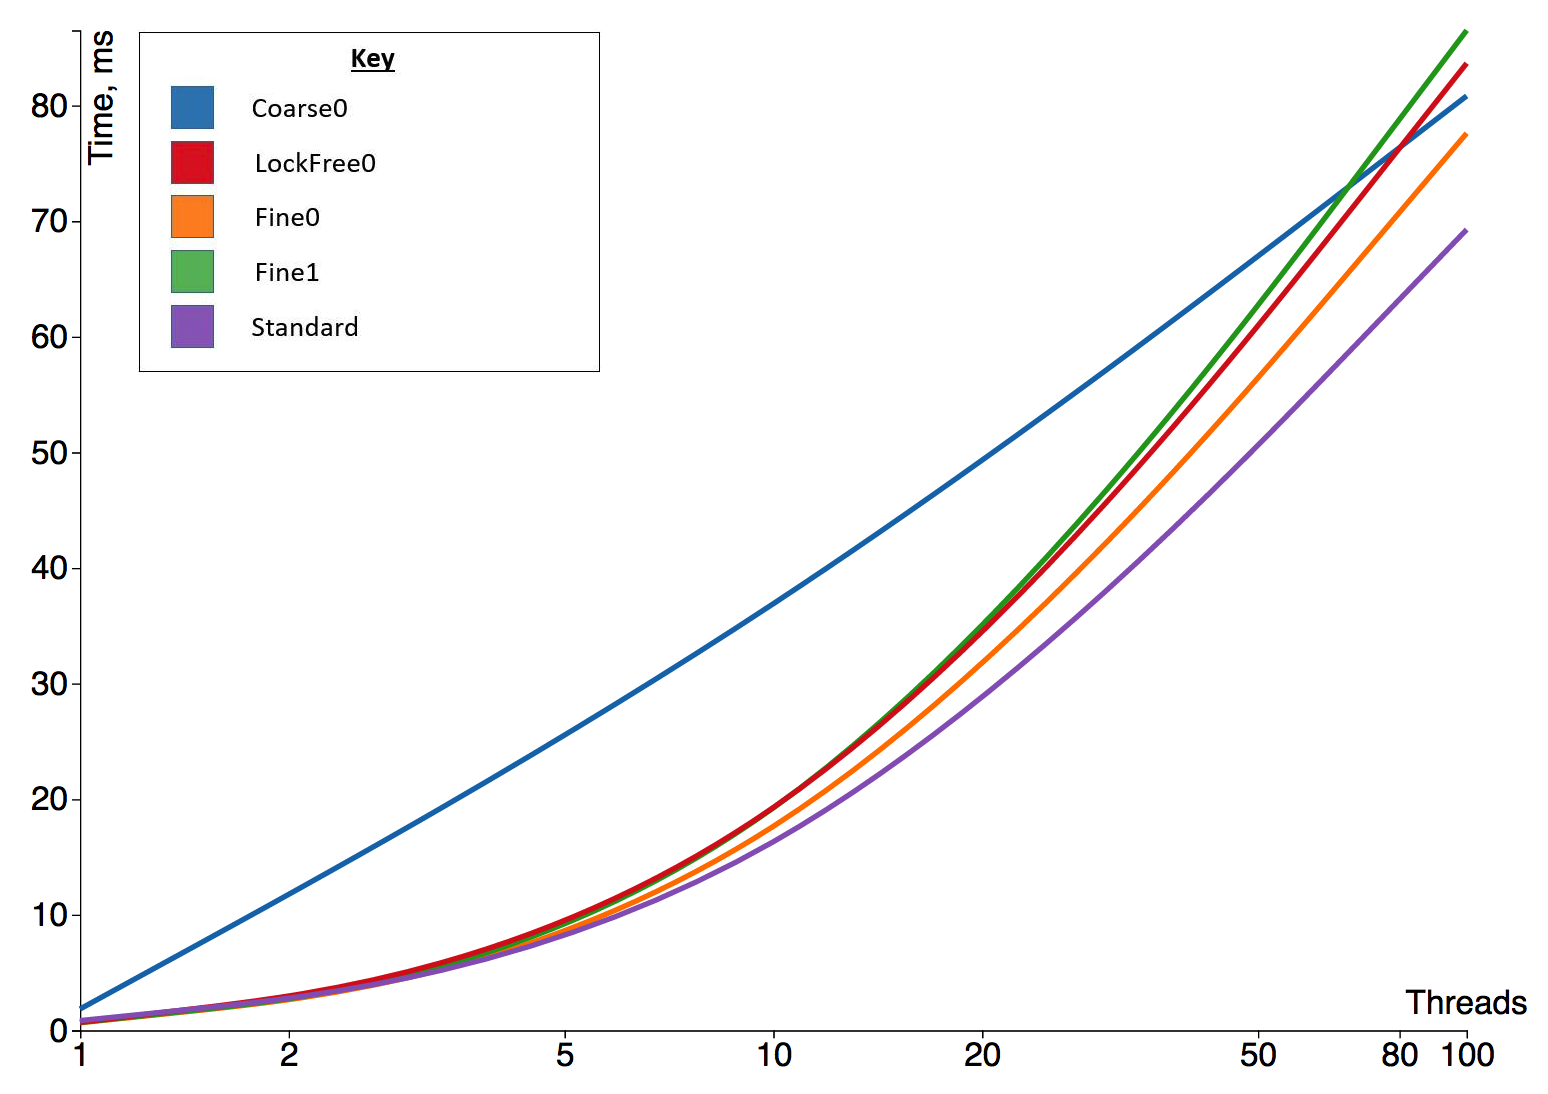
\includegraphics[width=0.37\linewidth]{11}\hspace{0em}
    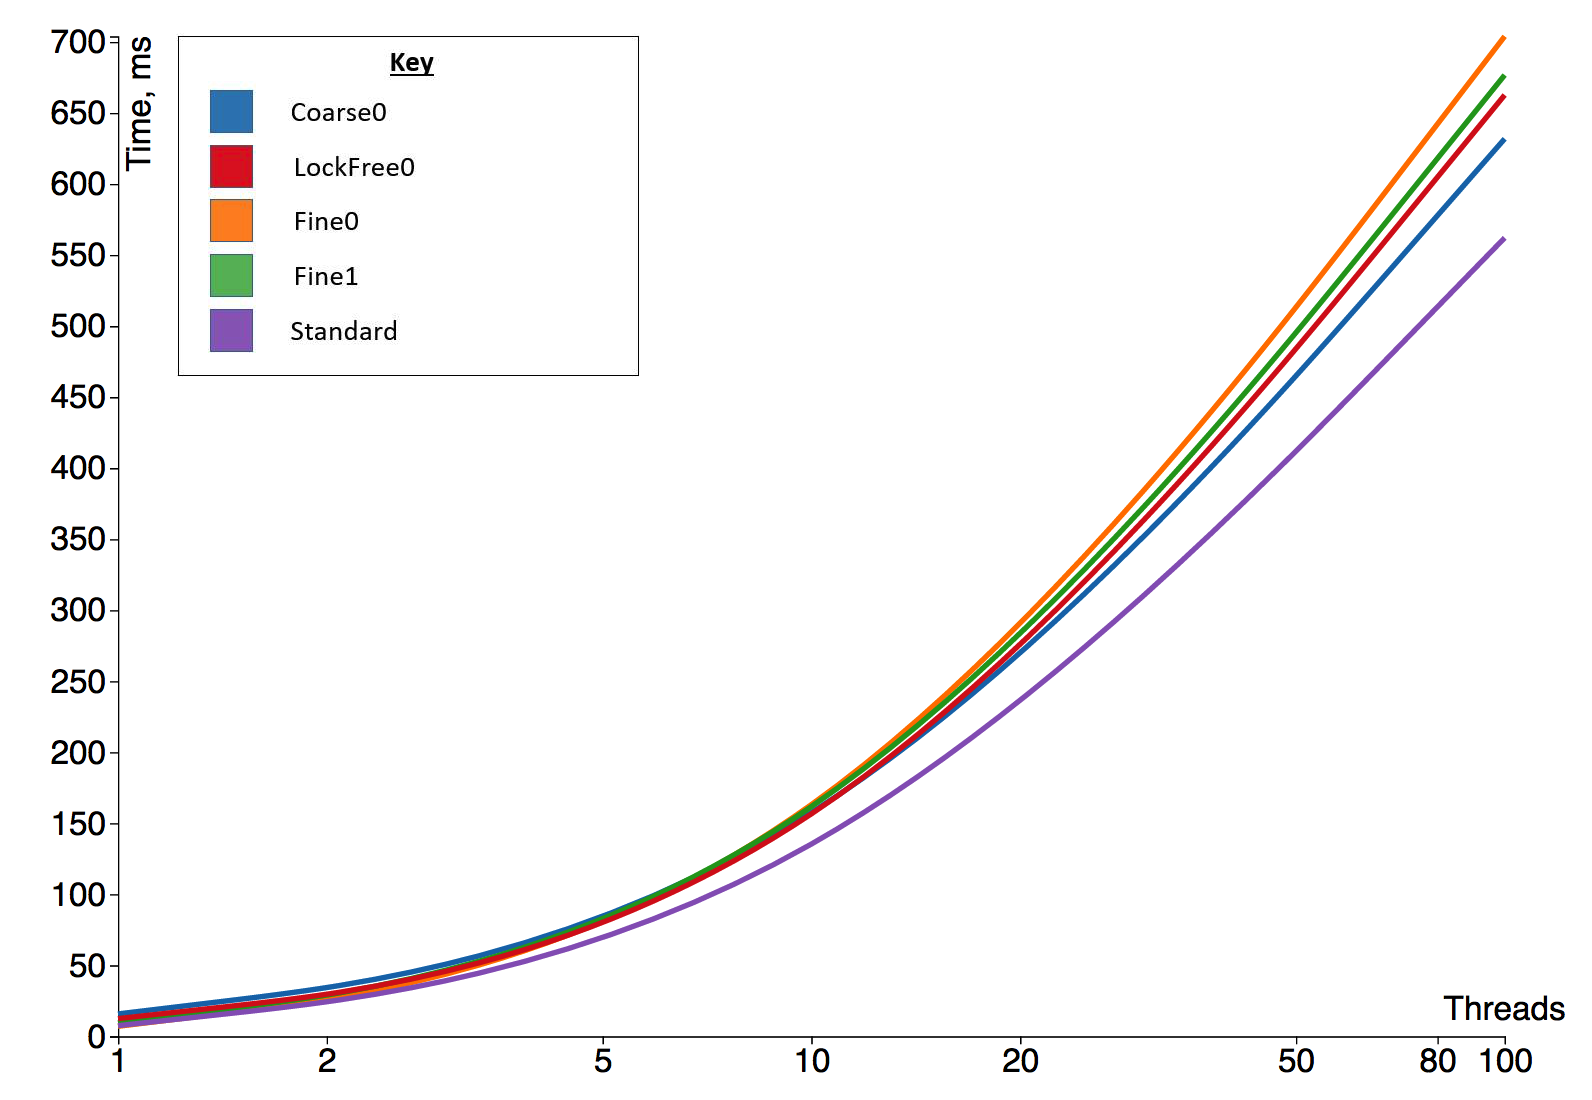
\includegraphics[width=0.37\linewidth]{12}
    \hspace*{-2.25cm}
    \centering
    \caption{Time v. number of threads (90\% get, 9\% add, 1\% remove operations). The same key is retrieved 50\% of the time.\newline{}
    {\it  From left-to-right: 10 operations, 100 operations, 1000 operations.}}
    \label{fig:g4}
\end{figure}

\section{Conclusion}

After executing performance benchmarks on our skiplist implementations, we found that our implementations were comparable even as the number of operations and number of threads grew large. In most cases, our non-optimized fine-grained implementation performed at least as well, if not better than, our coarse-grained implementation. We theorize that this is most probably due to the optimism and laziness strategies which are present in the fine-grained implementation. Secondly, we can claim that our lock-free implementation performed comparable to our non-optimized fine-grained implementation for 100 or more operations. Lastly, although our fine-grained and lock-free implementations performed better than the Java standard library {\tt ConcurrentSkipListMap} for 10 operations, we cannot conclude any definitive result from this since 10 operations is a small number.

% \begin{verbatim}
\begin{thebibliography}{0}
\bibitem{pugh1}
William Pugh. Skip Lists: A Probabilistic Alternative to Balanced Trees. Communications of the ACM, 33(6):668–676, June 1990 (p 47).
\bibitem{pugh2}
William Pugh. Concurrent Maintenance of Skip Lists. Technical Report CS-TR-2222, Department of Computer Science, University of Maryland, June 1990 (p 20, 47, 49, 63, 73, 86).
\bibitem{fraser}
Fraser, K. Practical Lock-Freedom. PhD thesis, University of Cambridge, 2004.
\bibitem{heller}
Heller, S., Herlihy, M., Luchangco, V., Moir, M., Shavit, N., and Scherer III, W. N. A lazy concurrent list-based set algorithm. In Proceedings of 9th International Conference on Principles of Distributed Systems, December 2005.
\bibitem{art}
M. Herlihy and N. Shavit. The Art of Multiprocessor Programming. Morgan Kaufmann, 2008. (p 339-348)
\bibitem{provably}
M. Herlihy, Y. Lev, V. Luchangco, and N. Shavit. A provably correct scalable concurrent skip list. In OPODIS ’06: Proceedings of the 10th International Conference On Principles Of Distributed Systems, 2006.
\end{thebibliography}
% \end{verbatim}














\clearpage


\section*{Appendix A: Data}

This appendix is a listing of the benchmarking results. The graphs are derived from these data points. The numbers represent the runtime in nanoseconds (averaged over 5 runs) for the specified number of threads for each skiplist implementation.

\subsection*{{0\%} get, 50\% add, 50\% remove}

{\tt
\begin{table}[htb]
    \begin{tabular}{llllll}
     threads & coarse0      & fine0        & fine1      & lockfree0    & standard     \\
    1        & 853978.0     & 878243.6     & 753604.8   & 931719.0     & 1003152.0    \\
    10       & 2781592.2    & 1951835.0    & 2031042.4  & 2743772.8    & 1.06397366E7 \\
    100      & 3.56624326E7 & 2.29277024E7 & 1.245763E7 & 3.05522982E7 & 2.16020812E7 \\
    ~        & ~            & ~            & ~          & ~            & ~            \\
    \end{tabular}
    \caption{{\rm numOps=10}}
\end{table}
}

{\tt
\begin{table}[htb]
    \begin{tabular}{llllll}
     threads & coarse0     & fine0       & fine1        & lockfree0    & standard     \\
    1        & 1328751.4   & 1630393.4   & 609803.8     & 1279606.0    & 908283.6     \\
    10       & 7663687.8   & 7856480.2   & 1.08999796E7 & 9730179.8    & 6927417.0    \\
    100      & 7.5545487E7 & 8.5041961E7 & 8.9512078E7  & 8.35204142E7 & 7.45853728E7 \\
    ~        & ~           & ~           & ~            & ~            & ~            \\
    \end{tabular}
    \caption{{\rm numOps=100}}
\end{table}
}

{\tt
\begin{table}[htb]
    \begin{tabular}{llllll}
     threads & coarse0       & fine0        & fine1         & lockfree0     & standard      \\
    1        & 4133202.8     & 4549592.6    & 5696434.8     & 6099599.6     & 4420815.2     \\
    10       & 7.2543509E7   & 6.12522908E7 & 6.22689446E7  & 6.06235896E7  & 4.69082802E7  \\
    100      & 6.418871744E8 & 5.99773773E8 & 5.909121142E8 & 6.449246182E8 & 5.607032962E8 \\
    ~        & ~             & ~            & ~             & ~             & ~             \\
    \end{tabular}
    \caption{{\rm numOps=1000}}
\end{table}
}




\clearpage
\subsection*{{70\%} get, 20\% add, 10\% remove}

{\tt
\begin{table}[htb]
    \begin{tabular}{llllll}
     threads & coarse0      & fine0        & fine1       & lockfree0    & standard     \\
    1        & 911714.4     & 485684.0     & 1019696.4   & 782988.6     & 663853.8     \\
    10       & 3293721.6    & 2062057.6    & 1627378.0   & 2136806.6    & 1799910.2    \\
    100      & 4.33736456E7 & 2.10236398E7 & 2.2747486E7 & 2.56547998E7 & 1.32812334E7 \\
    ~        & ~            & ~            & ~           & ~            & ~            \\
    \end{tabular}
    \caption{{\rm numOps=10}}
\end{table}
}

{\tt
\begin{table}[htb]
   \begin{tabular}{llllll}
     threads & coarse0      & fine0        & fine1        & lockfree0    & standard     \\
    1        & 583811.0     & 577628.8     & 579586.0     & 1194818.2    & 873634.4     \\
    10       & 8736083.2    & 8168063.2    & 6870574.4    & 6589303.0    & 6127142.8    \\
    100      & 8.46005466E7 & 7.78242122E7 & 7.94677586E7 & 8.02945156E7 & 6.83953066E7 \\
    ~        & ~            & ~            & ~            & ~            & ~            \\
    \end{tabular}
    \caption{{\rm numOps=100}}
\end{table}
}

{\tt
\begin{table}[htb]
    \begin{tabular}{llllll}
     threads & coarse0       & fine0         & fine1         & lockfree0     & standard      \\
    1        & 1.2118481E7   & 8777019.0     & 6509660.0     & 7997591.6     & 6388901.6     \\
    10       & 8.44526416E7  & 1.214440704E8 & 5.61010358E7  & 6.8482695E7   & 5.58750644E7  \\
    100      & 6.199936564E8 & 5.887688254E8 & 5.690875734E8 & 5.557499856E8 & 5.141559318E8 \\
    ~        & ~             & ~             & ~             & ~             & ~             \\
    \end{tabular}
    \caption{{\rm numOps=1000}}
\end{table}
}

\clearpage
\subsection*{{90\%} get, 9\% add, 1\% remove}

{\tt
\begin{table}[htb]
   \begin{tabular}{llllll}
     threads & coarse0      & fine0        & fine1        & lockfree0    & standard     \\
    1        & 975534.6     & 1243016.2    & 1280808.2    & 1246848.0    & 1297043.0    \\
    10       & 9279587.6    & 2515896.6    & 2271124.4    & 4988213.8    & 2.66461754E7 \\
    100      & 2.08653528E7 & 1.62768616E7 & 3.25403948E7 & 3.61657788E7 & 1.11821576E7 \\
    ~        & ~            & ~            & ~            & ~            & ~            \\
    \end{tabular}
    \caption{{\rm numOps=10}}
\end{table}
}

{\tt
\begin{table}[htb]
    \begin{tabular}{llllll}
     threads & coarse0      & fine0        & fine1        & lockfree0    & standard     \\
    1        & 638999.2     & 728303.8     & 646445.8     & 681568.2     & 646497.6     \\
    10       & 1.46338414E7 & 1.04176336E7 & 7834194.8    & 1.04206238E7 & 6477948.4    \\
    100      & 7.63091862E7 & 8.40070824E7 & 7.60776048E7 & 7.73890456E7 & 6.88778234E7 \\
    ~        & ~            & ~            & ~            & ~            & ~            \\
    \end{tabular}
    \caption{{\rm numOps=100}}
\end{table}
}


{\tt
\begin{table}[htb]
    \begin{tabular}{llllll}
     threads & coarse0      & fine0         & fine1         & lockfree0    & standard      \\
    1        & 1.89422628E7 & 9805100.8     & 6705396.6     & 1.02943142E7 & 8633986.0     \\
    10       & 7.40453642E7 & 6.70482656E7  & 6.0373275E7   & 7.1410341E7  & 5.88771512E7  \\
    100      & 6.48191333E8 & 5.360148284E8 & 6.686908832E8 & 5.5540802E8  & 4.987920704E8 \\
    ~        & ~            & ~             & ~             & ~            & ~             \\
    \end{tabular}
    \caption{{\rm numOps=1000}}
\end{table}
}

\clearpage
\subsection*{{90\%} get, 9\% add, 1\% remove (Get the same key 50\% of the time)}

{\tt
\begin{table}[htb]
   \begin{tabular}{llllll}
     threads & coarse0      & fine0        & fine1       & lockfree0    & standard     \\
    1        & 1691550.2    & 924239.4     & 801858.6    & 532592.4     & 486972.4     \\
    10       & 8999507.8    & 4969882.4    & 2502099.6   & 7046680.4    & 1.36424E7    \\
    100      & 3.12601826E7 & 1.37520696E7 & 3.4292865E7 & 1.81954448E7 & 3.26613184E7 \\
    ~        & ~            & ~            & ~           & ~            & ~            \\
    \end{tabular}
    \caption{{\rm numOps=10}}
\end{table}
}

{\tt
\begin{table}[htb]
    \begin{tabular}{llllll}
     threads & coarse0      & fine0        & fine1        & lockfree0    & standard     \\
    1        & 1843498.0    & 653489.8     & 681405.6     & 695536.6     & 843390.8     \\
    10       & 3.46879096E7 & 6907366.6    & 7068526.0    & 7825639.2    & 6940283.2    \\
    100      & 8.08297576E7 & 7.76031002E7 & 8.65032678E7 & 8.36541624E7 & 6.92697892E7 \\
    ~        & ~            & ~            & ~            & ~            & ~            \\
    \end{tabular}
    \caption{{\rm numOps=100}}
\end{table}
}


{\tt
\begin{table}[htb]
    \begin{tabular}{llllll}
     threads & coarse0      & fine0         & fine1         & lockfree0    & standard      \\
    1        & 1.57709552E7 & 7058997.6     & 9551645.8     & 1.24931452E7 & 7526325.4     \\
    10       & 7.433552E7   & 6.68675186E7  & 7.10000604E7  & 6.61031956E7 & 6.05722368E7  \\
    100      & 6.3182553E8  & 7.039460026E8 & 6.766970202E8 & 6.62642416E8 & 5.620964268E8 \\
    ~        & ~            & ~             & ~             & ~            & ~             \\
    \end{tabular}
    \caption{{\rm numOps=1000}}
\end{table}
}


\end{document}
